% !TeX root=main.tex
\chapter{روش حل مسئله}
\thispagestyle{empty}

برای این‌که نمونه‌های تقابلی ساخته شده هم شبکه را بیشتر به خطا بیندازند و هم از نظر انسان‌ها واقعی‌تر باشند، از شبکه‌ای به عنوان
\lr{Adv-GAN}
استفاده می‌شود.
\cite{Xiao2018GeneratingAE}

\section{شرح مسئله}
اگر موارد زیر را در نظر بگیریم:
\begin{itemize}
	\item $X \subseteq R^n$:
	فضای ویژگی
	\LTRfootnote{Feature Space}
	
	\begin{itemize} 
		\item n:
		تعداد ویژگی 
	\end{itemize}

	\item $(x_i, y_i)$:
	نمونه i ام در داخل مجموعه داده‌های آموزش که تشکیل شده است از بردارهای ویژگی
	\LTRfootnote{Feature Vectors}:
	\begin{itemize}
		\item $x_i \in X$:
		با توجه به یک توزیع ناشناخته‌ی
		\LTRfootnote{Unknown Distribution}
		$x_i \sim P_{data}$
		ساخته ‌می‌شوند.
		
		\item $y_i \in Y$:
		برچسب کلاس حقیقی و درست
	\end{itemize}
\end{itemize}
هدف سیستم یادگیرنده 
\LTRfootnote{Learning System}
این است که یک طبقه‌بند
\LTRfootnote{Classifier} 
$f: X \rightarrow Y$
را از دامنه
$X$
به مجموعه‌ی خروجی‌های دسته‌بندی 
$Y$
یادبگیرد.
\\ 
با دادن یک نمونه 
$x$
هدف حمله‌کننده این است که یک نمونه‌ متقابلی 
$x_A$
را تولید کند که به صورت 
$f(x_A) \neq y$
(در حمله بدون هدف)، و 
$f(x_A) = t$
(در حمله هدفمند) که 
$t$
کلاس هدف است، طبقه‌بندی شود.
\\
همچنین 
$x_A$
باید از نظر فاصله‌ی
$L^2$
یا سایر روش‌های سنجش فاصله به نمونه اصلی
$x$
نزدیک باشد.

\section{شبکه 
\lr{Adv-GAN}
}
این شبکه به این صورت است که از یک شبکه عصبی پیش‌خور
\LTRfootnote{Feed-Forward Neural Network}
برای تولید تغییرات جزئی و از یک شبکه تمییزدهنده برای اطمینان پیدا کردن از نزدیک به واقعیت بودن نمونه‌های تولید شده استفاده می‌شود.
\\
در مقایسه با روش علامت گرادیان سریع، در این روش، پس از آموزش شبکه پیش‌خور، بی‌درنگ و فورا می‌توان از آن برای تولید دستکاری‌های تقابلی برای هر نمونه‌ی ورودی، بدون نیاز به دسترسی به خود مدل (حمله جعبه نیمه‌سفید)، استفاده کرد.
\\
شبکه 
\lr{Adv-GAN}
این قابلیت را دارد که هم در حمله‌های جعبه نیمه‌سفید و جعبه سیاه و هم در حمله هدفمند و بدون هدف استفاده شود.

\subsection{معماری شبکه}
نمای کلی معماری شبکه
\lr{Adv-GAN}
در شکل 
\ref{advgan_arch}
به تصویر کشیده شده است. 
این شبکه دارای سه شبکه عصبی است:
\begin{enumerate}
	\item
	مولد $G$
	\item
	تمییزدهنده $D$
	\item
	شبکه عصبی هدف $f$
\end{enumerate}
مولد نمونه‌ اصلی 
$x$
را به عنوان ورودی می‌گیرد و یک دستکاری
$G(x)$
را تولید می‌کند. سپس 
$x + G(x)$
به تمییزدهنده
$D$
فرستاده می‌شوند که برای تمایز دادن بین نمونه تولید شده و نمونه اصلی استفاده می‌شود. در این‌جا نقش
$D$
به عنوان مشوق این است که نمونه‌های تولید شده از داده‌های کلاس اصلی غیر قابل تشخیص باشند.
در ادامه
$x + G(x)$
به عنوان ورودی به 
$f$
داده‌ می‌شود و ضرر 
$L_{adv}$
خود را مطابق فرمول
\ref{eq:f_loss}
به عنوان خروجی می‌دهد.
\cite{Xiao2018GeneratingAE} 
\\ 
\begin{figure}[H]
	\center{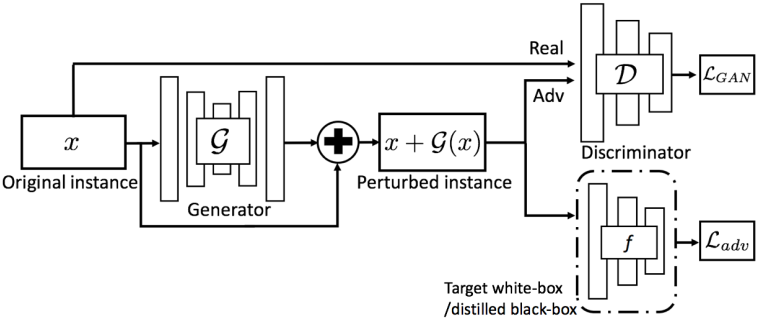
\includegraphics[width=\linewidth]{images/advgan_arch.PNG}}
	\caption{نمای کلی شبکه 
		\lr{Adv-GAN}
		\cite{Xiao2018GeneratingAE}}
	\label{advgan_arch}
\end{figure}

\subsection{معادله‌های شبکه}
در فرمول 
\ref{eq:gan_loss}
ضرر تقابلی
\LTRfootnote{Adversarial Loss}
آورده شده است:
\begin{equation} \label{eq:gan_loss}
	L_{GAN} = \mathbb{E}_x log D(x) + \mathbb{E}_x log (1- D(x + G(x)))
\end{equation}
فرمول 
\ref{eq:f_loss}
برای محاسبه ضرر برای فریب دادن مدل هدف 
$f$
در یک حمله هدفمند است:
\begin{equation} \label{eq:f_loss}
	L^f_{adv} = \mathbb{E}_x l_f(x + G(x), t)
\end{equation}
لازم به ذکر است که ضرر
$L^f_{adv}$
تصویر دستکاری شده را تشویق می‌کند که به اشتباه در کلاس هدف 
$t$
دسته‌بندی شود.
\\
برای محدود کردن اندازه دستکاری‌ها از یک ضرر
\lr{Soft Hinge}
 بر روی قاعده 
$L_2$
در فرمول 
\ref{eq:soft_hinge_loss}
استفاده می‌شود که در آن 
$c$
نشان دهنده‌ی محدودیتی است که توسط کاربر تعیین ‌می‌شود
\LTRfootnote{User-Specified Bound}:
\begin{equation} \label{eq:soft_hinge_loss}
	L_{hinge} = \mathbb{E}_x\:max(0, \|G(x)\|_2 - c)
\end{equation}

بنابراین در مجموع هدف نهایی در فرمول 
\ref{eq:total_loss}
آورده شده است:
\begin{equation} \label{eq:total_loss}
	L = L^f_{adv} + \alpha L_{GAN} + \beta L_{hinge}
\end{equation}
پارامترهای $\alpha$ و $\beta$ متناسب با اهمیت هر یک از اهداف هستند.
\\
در نهایت $D$ و $G$ با حل شدن یک بازی کمین‌بیش
\LTRfootnote{MinMax Game}
که در فرمول 
\ref{eq:minmax_advgan}
آورده شده است، بدست می‌آیند.
\begin{equation} \label{eq:minmax_advgan}
	arg\:min_G\:max_D\:L
\end{equation}
